\chapter{Experiments}
\label{cha:chapter4}


\section{General Setting}\label{sec:setup}
 
 We use \textit{Adaptive Moment Estimation(Adam)}\cite{KingmaAdamMethodStochastic2014} to train models and initialize weights $w_{ij} \in \patmatrix{W}$ and biases $b_{j} \in \patvector{b}$ as follows:
\begin{align*}
	w_{ij} &\sim \Psi( \mu, \sigma, [-2\sigma, 2\sigma]) \\
	b_{j} &= \ln(e^{0.01} - 1)
\end{align*}
where $\Psi(\cdot)$ denotes Truncated Normal Distribution where $\mathbb{P}(|w_{ij}| > 2\sigma) = 0$. Precisely, we use $\mu=0$ and $\sigma = 1/\sqrt{|\boldsymbol{a}|}$ where $|\boldsymbol{a}|$ is a number of neurons in previous layer.

The activations of neurons in layer $j$, denoted as $\patvector{a}^{(j)}$, are computed using :
\begin{align*}
\patvector{h}^{(j)}  &=  	(\patmatrix{W}_{ i \rightarrow j })^T \patvector{a}^{(i)} - \sigma_{s}(\patvector{b_j}) \\
	\patvector{a}^{(j)}  &=  	\sigma_{r} (	\patvector{h}^{(j)} )
\end{align*}

where $\sigma_r(\cdot)$ and $\sigma_s(\cdot)$ are \textit{ReLU} and \textit{softplus} function respectively and applied element-wise to the vectors.

 \begin{figure}[!hbt]
\centering
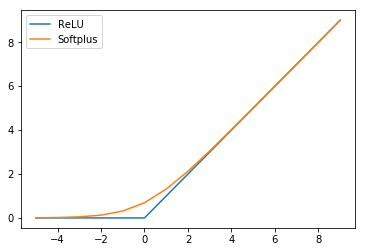
\includegraphics[width=0.5\textwidth]{relu_softplus}
\caption{ReLU and Softplus function} 
\label{fig:relu_softplus}
\end{figure}


The reason of using softplus function for the bias term is due to the non positive bias assumption of DTD. Moreover, because of the continuity of softplus function, bias term can be more flexibly adjusted through back-propagation than using  ReLU. With this setting, the initial value of bias term  $\sigma_{s}(b_j)$ is then 0.01.


\begin{table}[!htb]
\centering
\begin{tabular}{l|r}
\textbf{Hyperparameter} & \multicolumn{1}{l}{\textbf{Value}} \\ \hline
Optimizer               & Adam                               \\
Epoch     & 100                                \\
Dropout Probability     & 0.2                               \\
Batch size              & 50                                
\end{tabular}
\caption{Hyperparameter Summary}
\label{tab:hyper_summary}
\end{table}


\begin{table}[h]
\centering
\begin{tabular}{ll}
\multicolumn{1}{l|}{\textbf{Dataset}} & \textbf{Minimum Accuracy} \\ \hline
\multicolumn{1}{l|}{MNIST}            & \multicolumn{1}{r}{98.00\%}  \\
\multicolumn{1}{l|}{FashionMNIST}    & \multicolumn{1}{r}{85.00\%}  \\
%\multicolumn{1}{l|}{UFI Cropped}                                       &                         \dots
\end{tabular}
\caption{Minimum Classification accuracy for models to be considered}
\label{tab:min_acc}
\end{table}



Dropout technique \cite{SrivastavaDropoutSimpleWay2014} is applied to activations of every fully-connected layer, unless stated otherwise,  with the probability at 0.2. We train models with batch size 50 for 100 epochs. Table \ref{tab:hyper_summary} summaries the setting of hyperparameters. On the other hand, Learning rate is not globally fixed and left adjustable per architecture: the value varies between 0.0001 and 0.0005. Based on literature surveys, Table \ref{tab:min_acc} shows minimum accuracy for models to be used in the following experiments.  Numbers of neurons in each layer were carefully chosen such that every architecture has similar number of trainable variables. More precise configuration will be discussed separately in each experiment. 

Denote $g_r$ and $g_{f}$ function that a RNN with $\boldsymbol{\theta} = \{ \patmatrix{W}, \boldsymbol{b} \}$ uses to compute recurrent input $\patvector{r}_{t+1}$ and $f(\x)$ respectively. For a classification problem with $K$ classes, the calculations can be  roughly summarized as follows: 
 \begin{align*}
 	\patvector{r}_{t+1} &= g_r(\patvector{\theta}, \patvector{x_t}, \patvector{r_t}) \\
 	 &\ \ \vdots\\
f(\x) &= g_{f}(\patvector{\theta}, \patvector{x}_{T},  \patvector{r}_{T}) \\
 	\patvector{\hat{y}} &= \text{softmax}(f(\x)),
 \end{align*}
 where $t \in \{1, \dots, T\}$, $(\x_t \in \x)_1^{T}$ are the input corresponding to  step $t$, $\patvector{r}_0 = \patvector{0}$, and $\patvector{\hat{y}} \in \mathbb{R}^K$ are the class probabilities. To compute explanation or relevance heatmap of $\x$, denoted as $R(\x)$, we take $z^* \in f(\x)$ that is corresponding to the true target class, instead of the predicted class.  Because DTD and LRP method are primarily  based on distributing positive relevance, we also introduce a constant input to softmax function with value zero to force building positive relevance, $z^* \in \mathbb{R}^+$. Mathematically, this constant does not affect the training procedure.

Our implementation is written in Python and TensorFlow\cite{AbadiTensorFlowLargeScaleMachine2016}. It is also publicly available on Github\footnote{\url{https://github.com/heytitle/thesis-designing-recurrent-neural-networks-for-explainability/releases/tag/release-final}}.  We run our experiments either on a GeForce GTX 1080 provided by TUB ML group or AWS's p2.xlarge\footnote{\url{https://aws.amazon.com/ec2/instance-types/p2/}} instance. It approximately takes 2 hour to train a model. 


% \todo{computational resource}
% \todo{Tensoflow Python and Repo}

 
 % 
%Traditionally, number of neurons in each layer ($n^{(l)}$) is  another hyperparameter that we can adjust. However, as the goal is to compare relevance heatmaps from different architectures, those numbers are fixed and chosen in such a way that total number of variables in each architecture are equivalent. \addfigure{\ref{fig:neuron_numbers}} illustrates the details of the settings.
%
%\begin{figure}[!htb]
%\centering
%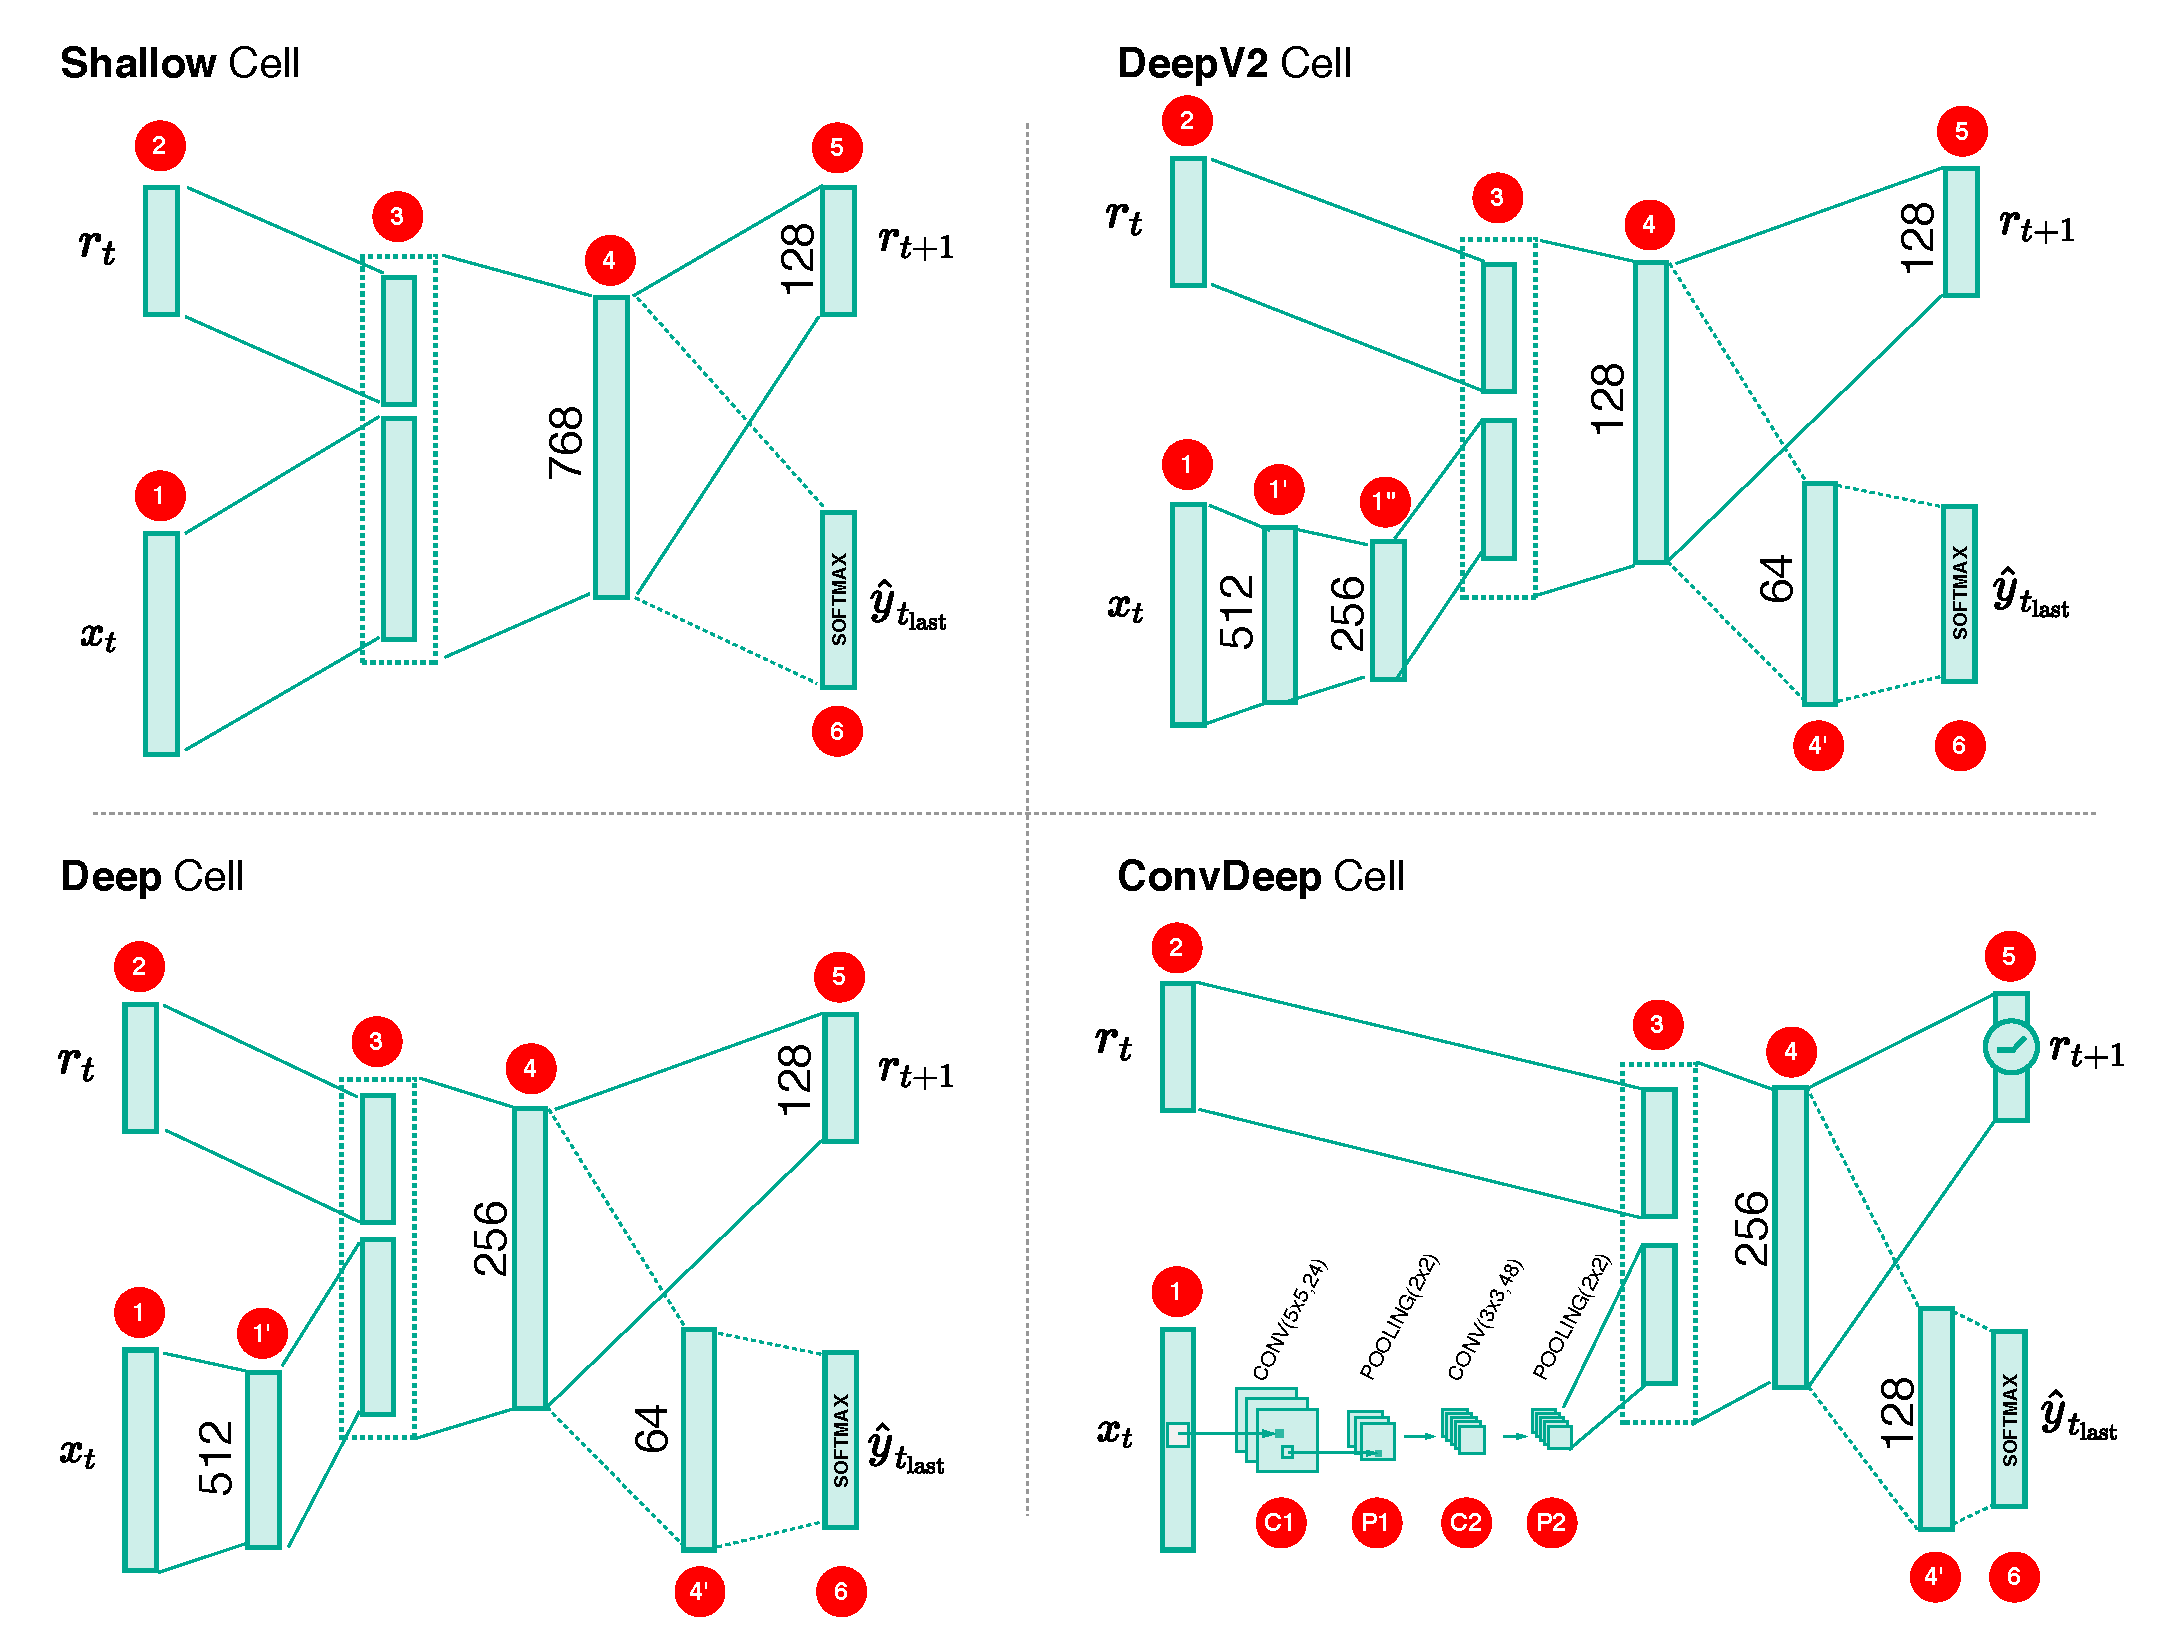
\includegraphics[width=\textwidth]{sketch/neuron_numbers}
%\caption{Number of neurons in each layer for each cell architecture}
%\label{fig:neuron_numbers}
%\end{figure}
%
%
%\begin{itemize}
%	\item \textbf{Shallow Cell} 
%$$\{ n^{(4)}\} = \{ 768 \}$$
%	\item \textbf{Deep Cell} 
%$$\{ n^{(1')}, n^{(4)}, n^{(4')} \} = \{ 512, 256, 64 \}$$
%	\item \textbf{DeepV2 Cell} 
%$$\{ n^{(1')}, n^{(1")}, n^{(4)}, n^{(4')} \} = \{ 512, 256, 128, 64 \}$$
%	\item \textbf{ConvDeep Cell} : 
%\begin{align*}
%	\{ n^{(C1)}, n^{(P1)} \} &= \{ CONV(5\text{x}5, 24), POOL(2\text{x}2) \} \\
%		\{ n^{(C2)}, n^{(P2)} \} &= \{ CONV(3\text{x}3, 48), POOL(2\text{x}2) \} \\
%			\{  n^{(4)}, n^{(4')} \} &= \{ 256, 128 \}
%\end{align*}
%where $CONV(x,y)$ is a convolutional operator with $y$ filters whose kernel size is $\mathbb{R}^{x}$. Similarly, $POOL(x)$ is a pooling operator  with kernel size $\mathbb{R}^{x}$.
%
%
%\end{itemize}
%
%Noting that, $n^{(5)}$ is set at 128 for all architectures and 0 when the sequence length of the problem is 1. $n^{(6)}$ is equal to the number of categories of a problem, for example $n^{(6)} = 10 $ MNIST. Table \ref{tab:variable_architecture} shows the total numbers of variables in details.

%\renewcommand{\arraystretch}{1.2}
%\begin{table}[h]
%\centering
%\begin{tabular}{l|c|c|c|}
%\cline{2-4}
%                                                 & \multicolumn{3}{c|}{\textbf{Sequence Length}} \\ \hline
%\multicolumn{1}{|l|}{\textbf{Cell Architecture}} & 1         & 4         & 7         \\ \hline
%\multicolumn{1}{|l|}{\rnncell{Shallow}}                    & 610570    & 355722    & 291210      \\ \hline
%\multicolumn{1}{|l|}{\rnncell{Deep}}                       & 550346    & 314954    & 271946      \\ \hline
%%\multicolumn{1}{|l|}{\rnncell{DeepV2}}                    & 575050    & 306890    & 263882      \\ \hline
%%\multicolumn{1}{|l|}{\rnncell{ConvDeep}}                   & 647594    & 283178    & 197162      \\ \hline
%\end{tabular}
%\caption{Total variables in each architecture and sequence length}
%\label{tab:variable_architecture}
%\end{table}


 

\clearpage
\section{Experiment 1 : Sequence Classification}
\label{sec:exp1}

\subsection{Problem Formulation}
In this preliminary experiment, we constructed an artificial classification problem in which each image sample $\x$ is column-wise split into a sequence of non-overlapping $(\x_t)_{t=1}^{T}$. The RNN classifier needs to summarize information from the sequence $(\x_t)_{t=1}^{T}$ to answer what is the class of $\x$.   Using image allows us to conveniently inspect how well RNNs can distribute relevant quantities to input space. 

\addfigure{\ref{fig:artificial_problem}} illustrates the setting. Here, a MNIST sample $ \patvector{x} \in \mathbb{R}^{28,28}$ is divided to a sequence of $( \patvector{x}_t \in   \mathbb{R}^{28,7} )_{t=1} ^ 4$. At time step $t$, $\patvector{x}_t$ is presented to the RNN classifier yielding recurrent input $\patvector{r}_{t+1}$ for the next step. For the last step $T$, in this example $T = 4$, the RNN classifier computes $f(\x) \in \mathbb{R}^{10}$ and class probabilities accordingly.


 \begin{figure}[!hbt]
		\centering
		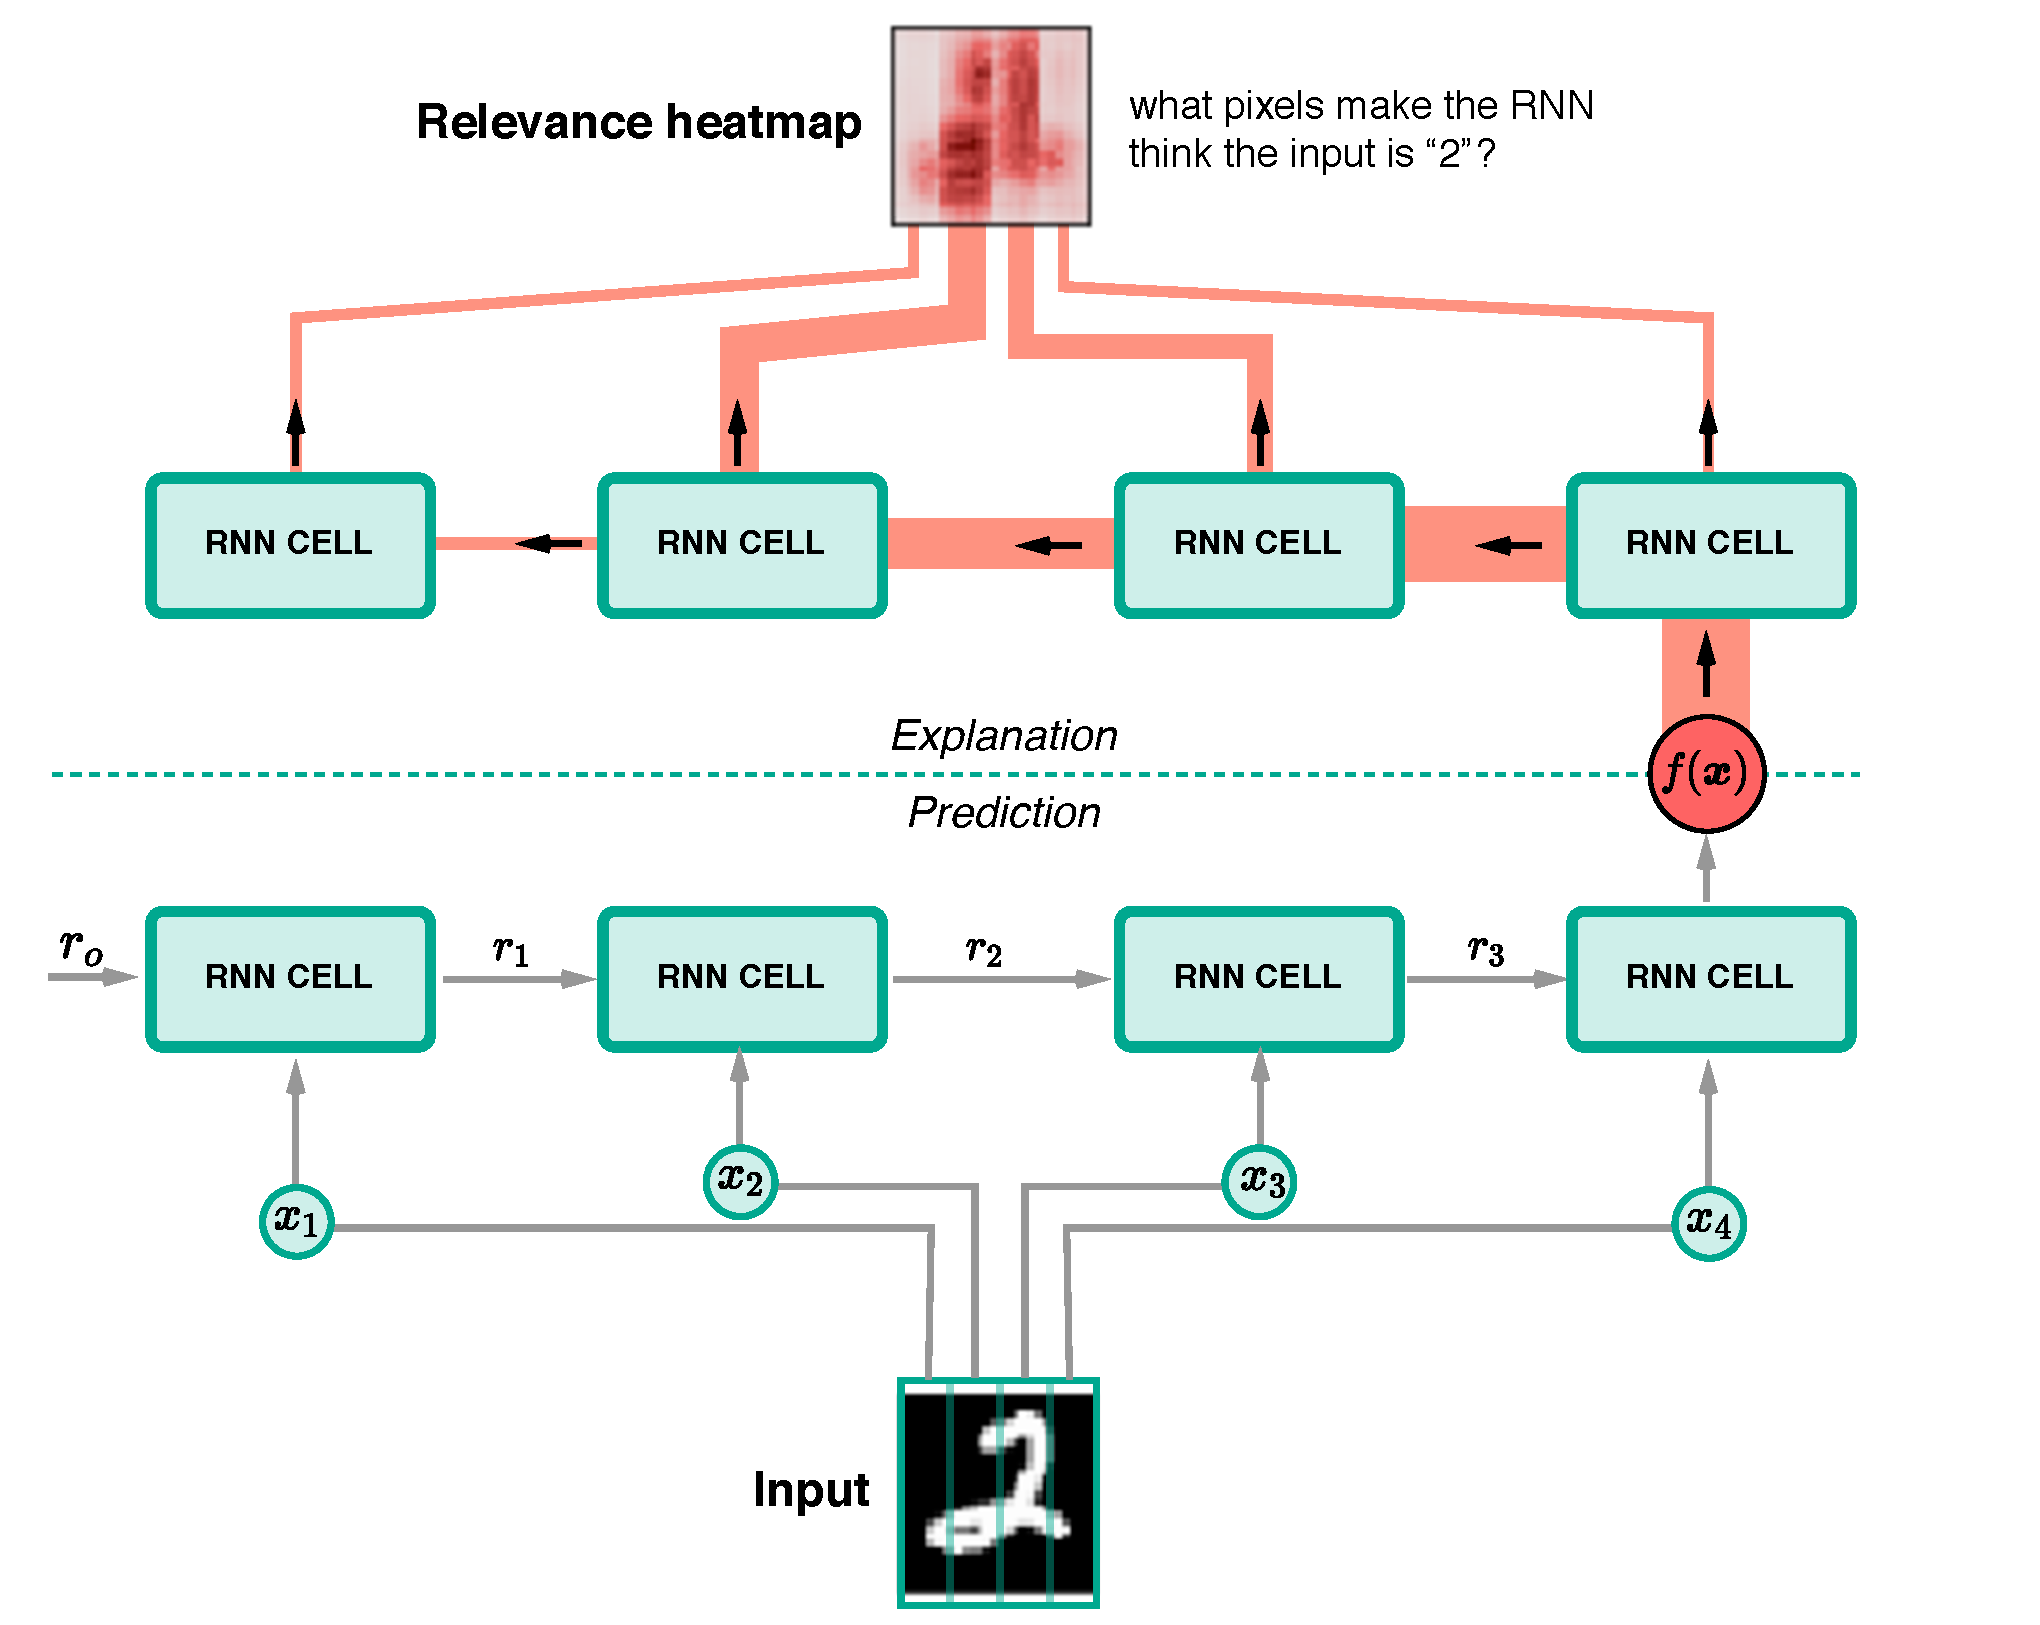
\includegraphics[width=\textwidth]{sketch/artificial_problem_with_rel}
		\caption{RNN Sequence classifier and decision explanation} 
		\label{fig:artificial_problem}
\end{figure}


\begin{figure}[!htb]
\centering

\subfloat[Shallow cell\label{fig:shallow_arch}]{%
       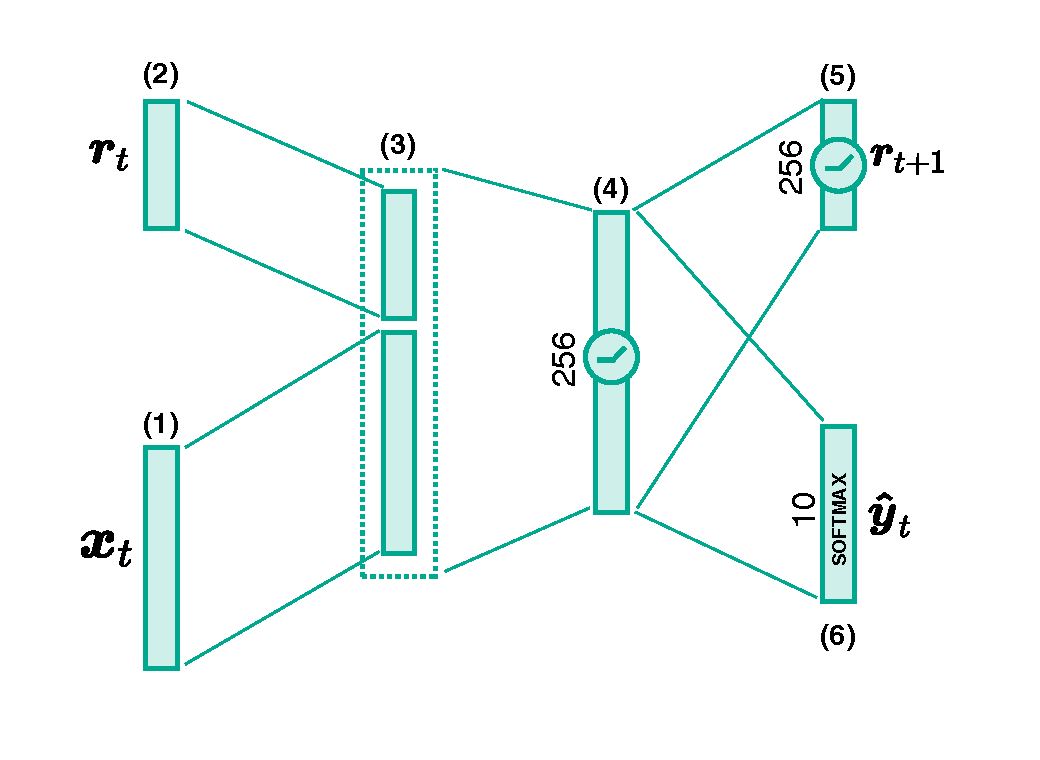
\includegraphics[width=0.48\textwidth]{sketch/shallow_arch}
     }
     \hfill
     \subfloat[Deep cell\label{fig:deep_arch}]{%
       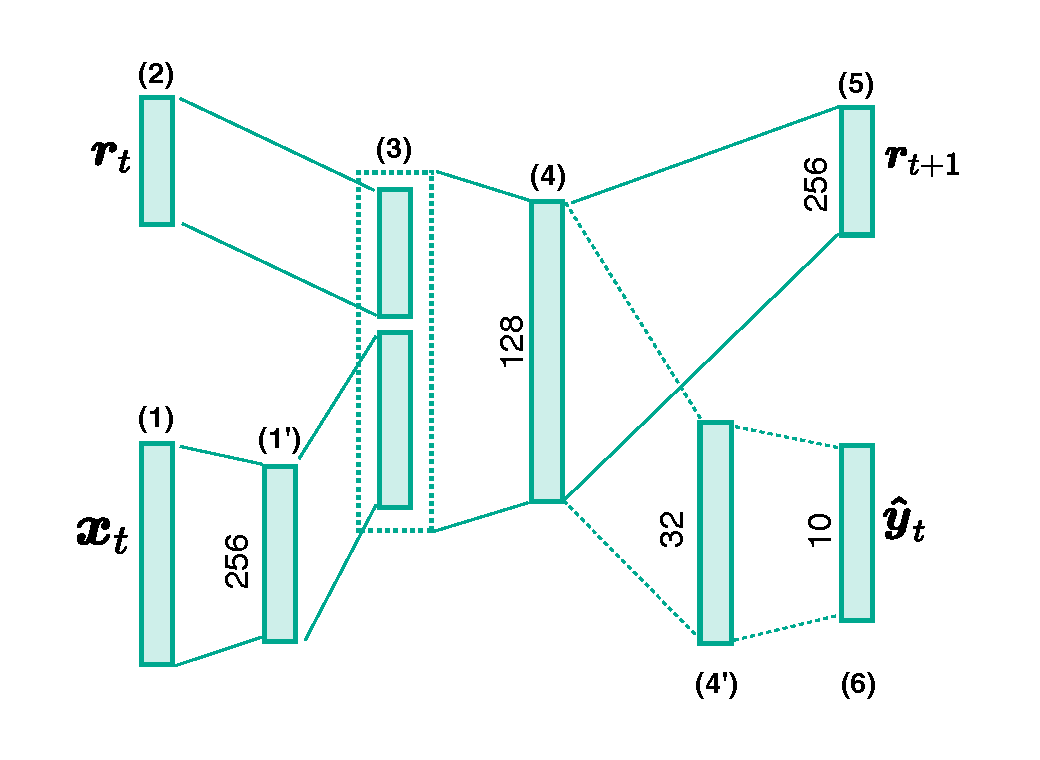
\includegraphics[width=0.48\textwidth]{sketch/deep_arch}
     }
\caption{Shallow and Deep cell architecture with number of neurons at each layer depicted.}
\end{figure}

We are considering to 2 cell architectures in this experiment, namely 

\begin{enumerate}
	\item \textbf{Shallow cell} \\
		As shown in \addfigure{\ref{fig:shallow_arch}}, the \rnncell{Shallow} cell first concatenates  input $\patvector{x}_t$  and recurrent input $\patvector{r}_t$ at layer \circled{3} as one vector before computing activations of layer \circled{4}, denoted as $\patvector{a}_t^{(4)}$. Then,  the next recurrent input $\patvector{r}_{t+1}$ \circled{5}	 is derived from $\patvector{a}_t^{(4)}$. In the last step $T$, $f(\x)$ is computed from $\patvector{a}^{(4)}_{T}$ and applied to softmax function to compute class probabilities $\patvector{\hat{y}}$. \todo{Adpated LRP rules for mixed domain propagation}
	\item \textbf{Deep cell} \\
		\addfigure{\ref{fig:deep_arch}} illustrates the architecture of  the \rnncell{Deep} cell. Unlike the Shallow architecture, the Deep cell has 2 more layers, namely \circled{1'} and \circled{4'}.  The idea is to let \circled{1'} learn representations of the input, while \circled{4} can focus on combining information from the past and current input. This then enables \circled{4'} to compute more fine-grained decision probabilities. 
\end{enumerate}

\renewcommand{\arraystretch}{1.5}
\begin{table}[h]
\centering
\begin{tabular}{cc|c|c|}
\cline{3-4}
& & \multicolumn{2}{c|}{\textbf{No. trainable variables}}                                                                \\ \hline
\multicolumn{1}{|c|}{\textbf{T}}               & \multicolumn{1}{c|}{\textbf{Dim. of $\x_t$}} & \multicolumn{1}{c|}{\textbf{Shallow}} & \multicolumn{1}{c|}{\textbf{Deep}}  \\ \hline
\multicolumn{1}{|c|}{1} & $\mathbb{R}^{28,28}$ & 269,322  &  271,338 \\
\multicolumn{1}{|c|}{4} & $\mathbb{R}^{28,7}$ & 184,330 & 153,578 \\
\multicolumn{1}{|c|}{7} & $\mathbb{R}^{28,4}$ & 162,826 & 132,074 \\ \hline

\end{tabular}
\caption{Dimensions of $\patvector{x}_t$ and number of trainable variables in each cell architecture on sequence length $T=\{1, 4, 7\}$.}
\label{tab:seq-length}
\end{table}
\renewcommand{\arraystretch}{1}




We experimented with MNIST and FashionMNIST data using sequence length $T = \{1, 4, 7\}$.  Table \ref{tab:seq-length} shows dimensions of $\patvector{x}_t$ for different sequence length as well as number of trainable variable in each architecture.

To simplify the writing, we am going to use \textit{\rnncellseq{ARCHITECTURE}{T}} convention to denote a RNN with \textit{ARCHITECTURE} trained on the sequence length \textit{T}. For example, \rnncellseq{Deep}{7} refers to the Deep cell trained on $(\x_t \in \mathbb{R}^{28,4} )_{t=1}^{7}$.

\subsection{Result}
\label{sec:exp1_result}

\renewcommand{\arraystretch}{1.5}
\begin{table}[]
\centering
\begin{tabular}{cc|c|c|c|}
\cline{2-5}
& \multicolumn{2}{|c|}{\textbf{MNIST}} & \multicolumn{2}{|c|}{\textbf{FashionMNIST}} \\ \hline
\multicolumn{1}{|c|}{$T$}   & \multicolumn{1}{c|}{\textbf{Shallow}} & \multicolumn{1}{c|}{\textbf{Deep}} & \multicolumn{1}{c|}{\textbf{Shallow}} & \multicolumn{1}{c|}{\textbf{Deep}} \\ \hline
\multicolumn{1}{|c|}{1} & 98.11\%   & 98.22\% & 87.93\%  & 89.14\%                           \\
\multicolumn{1}{|c|}{4} & 98.56\% & 98.63\%  & 89.04\%  & 89.43\%                            \\
\multicolumn{1}{|c|}{7} & 98.66\%  & 98.68\% & 89.28\%  & 88.96\%  \\ \hline
\end{tabular}
\caption{Accuracy of models trained for sequence classification problem with different sequence lengths and dataset. }
\label{tab:mnist_model_acc}
\end{table}
\renewcommand{\arraystretch}{1}



 \begin{figure}[!htb]
\centering
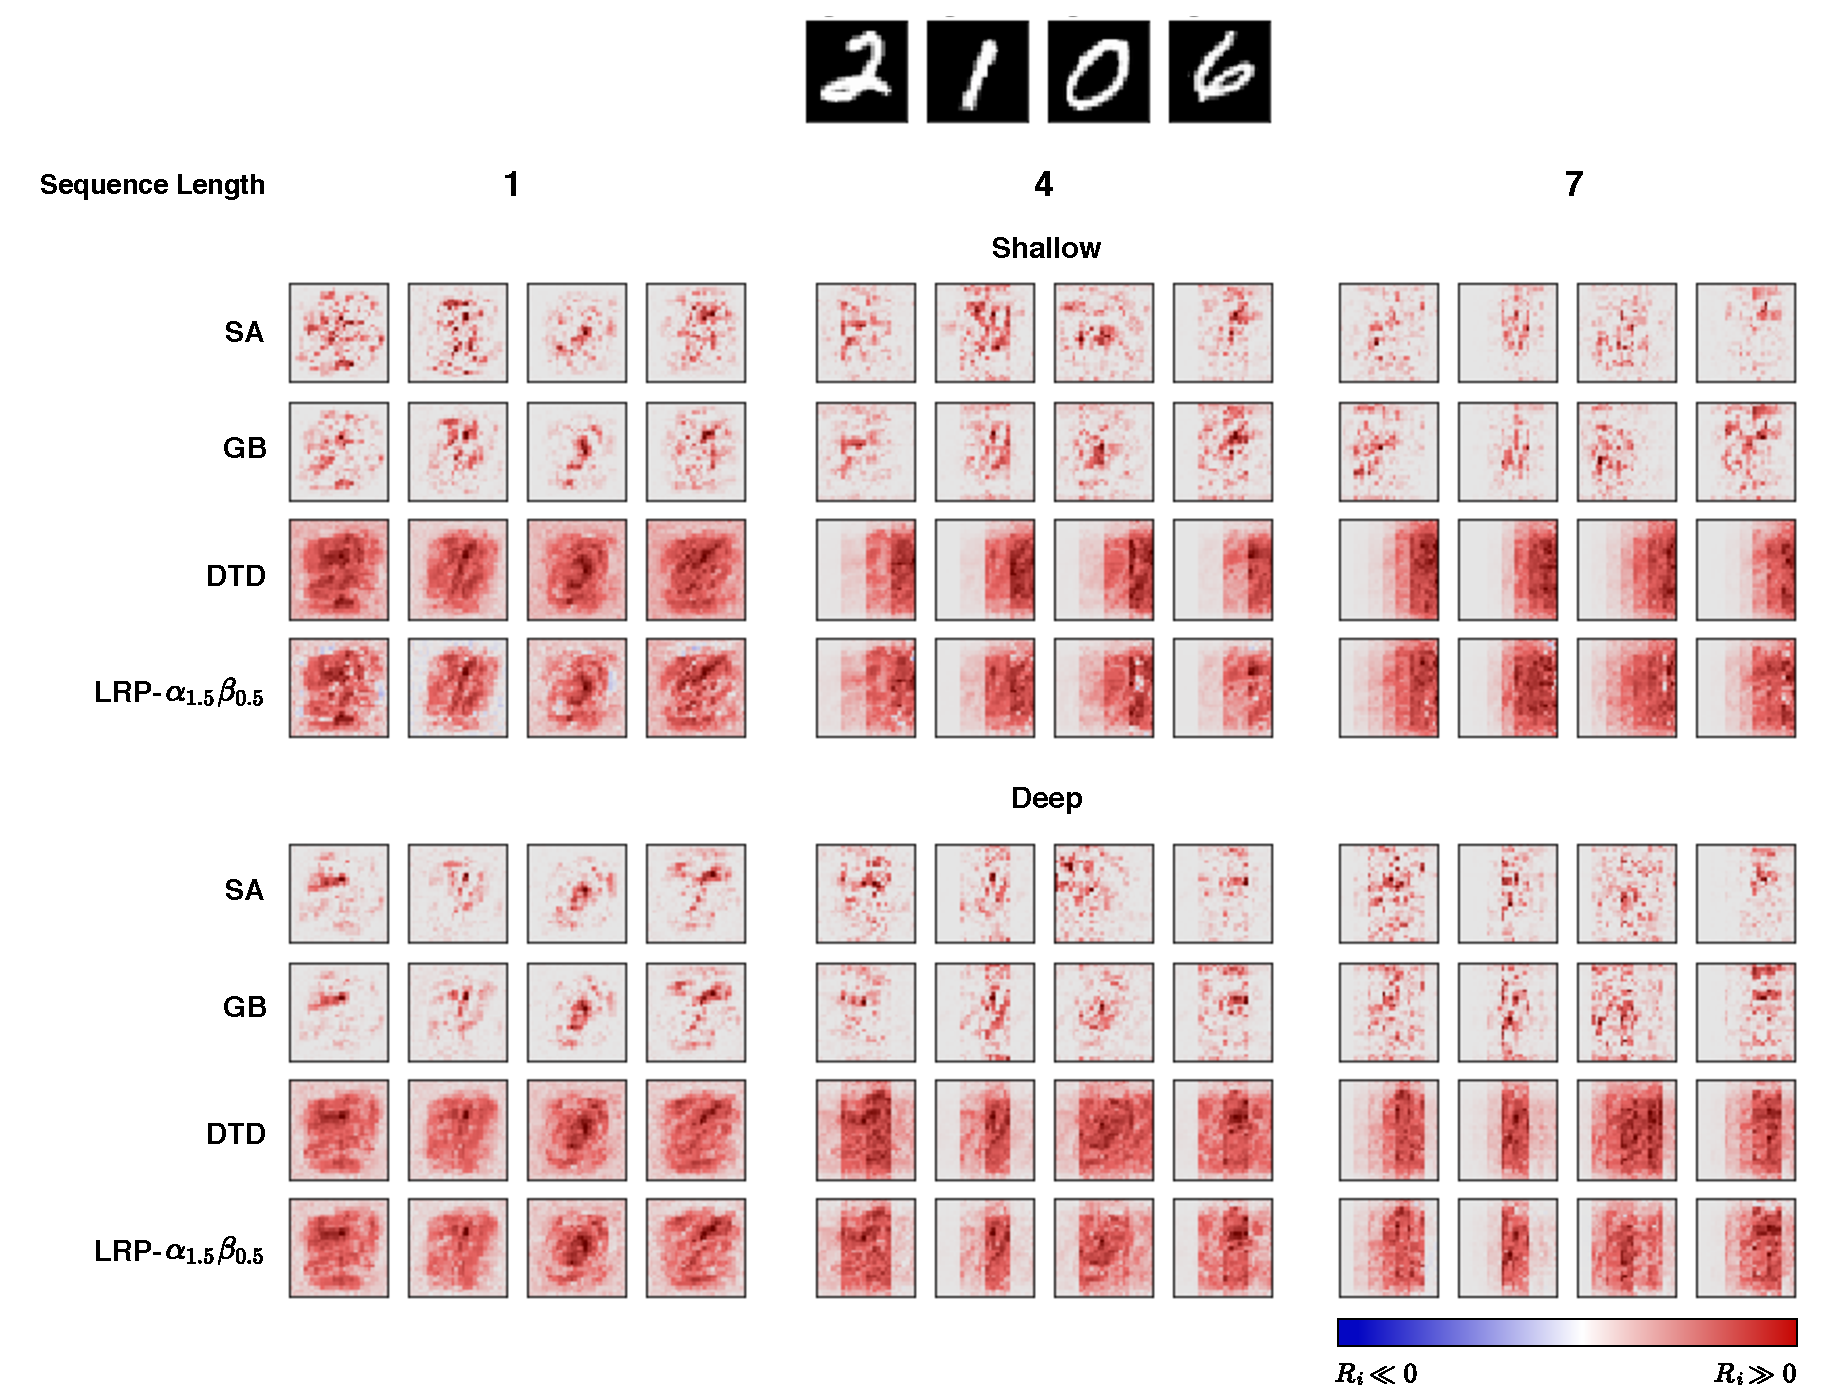
\includegraphics[width=0.8\textwidth]{sketch/mnist_experiment}
\caption{Relevance heatmaps produced by different explanation techniques of Shallow and Deep architecture trained on MNIST with different sequence lengths. \heatmapscaleexplain }
\label{fig:mnist_experiment}
\end{figure}


Table \ref{tab:mnist_model_acc} summaries accuracy of the trained models. Both Shallow and Deep architecture have comparable accuracy, hence their explanations can also be compared. \addfigure{\ref{fig:mnist_experiment}} shows relevance heatmaps from Shallow and Deep architecture trained on MNIST.  We can observe general characteristics of each explanation technique. In particular, sensitivity analysis(SA) and guided backprop(GB) heatmaps are sparse, while the ones from deep Taylor decomposition(DTD) and Layer-Wise Relevance Propagation (LRP) are more diffuse throughout $\x$. 

 When applying these techniques to \rnncellseq{Shallow}{1}  and \rnncellseq{Deep}{1}, the relevance heatmaps look similar regardless of the architectures.  As the sequence length is increased, SA and GB heatmaps are still almost identical  for \rnncellseq{Shallow}{4} and \rnncellseq{Deep}{4} as well as their 7-sequence length pair. However, this is not the case for DTD and LRP.  From the figure, we can see that \rnncellseq{Shallow}{4,7} and  \rnncellseq{Deep}{4,7} produce significantly different relevance heatmaps when  being explained by DTD and $\lrpp$ method.  In particular,  \rnncellseq{Shallow}{4,7} 's heatmaps are mainly concentrated on the right part of $\x$ associating to last time steps, while  \rnncellseq{Deep}{4,7}'s ones are proportionally  highlighted around content area of $\x$.


 \begin{figure}[!htb]
\centering
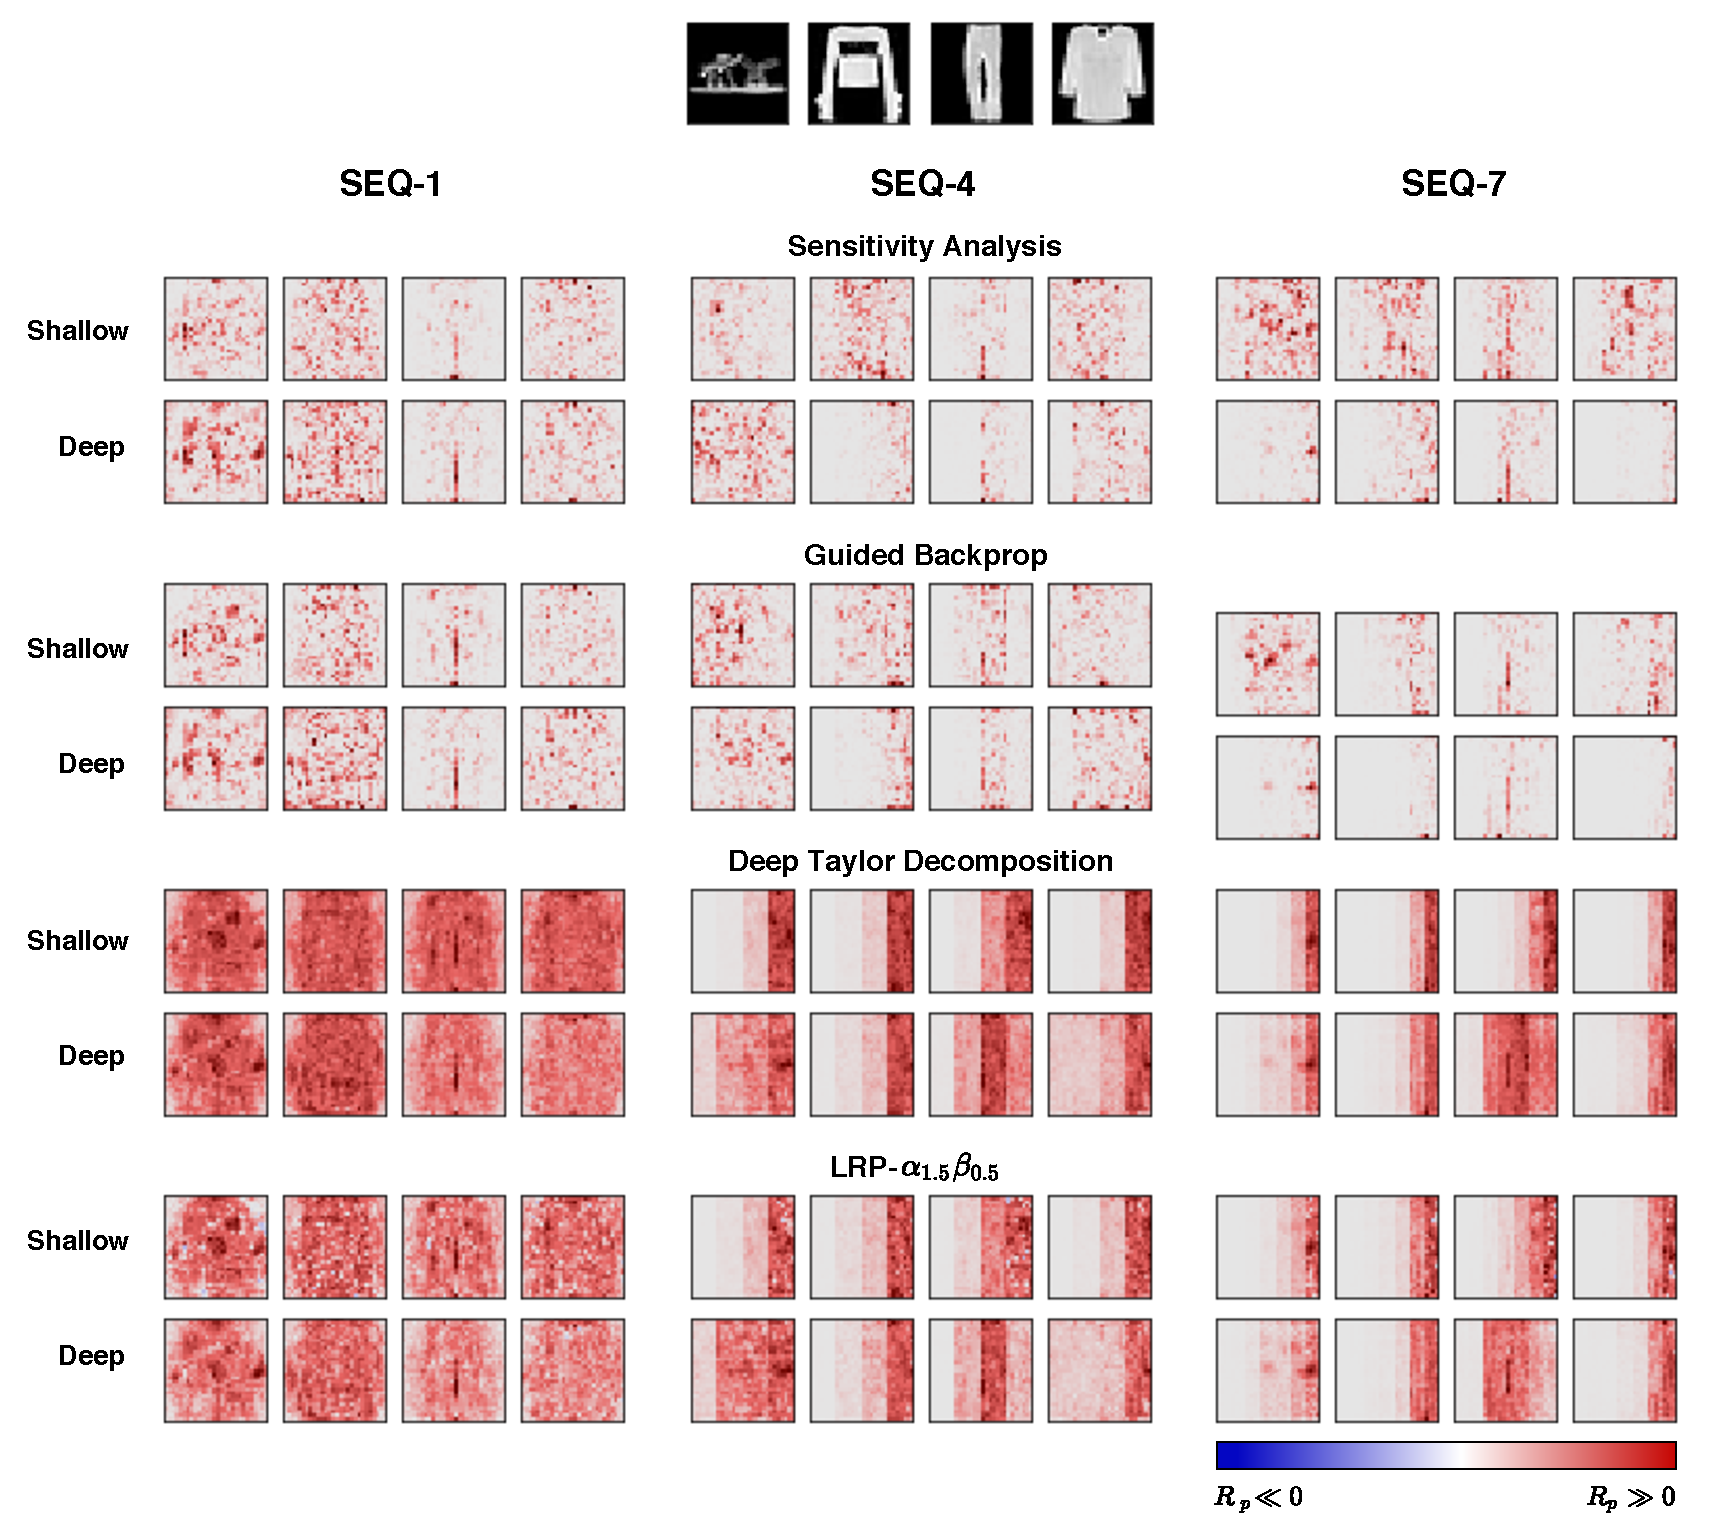
\includegraphics[width=0.8\textwidth]{sketch/fashion_mnist_experiment}
\caption{Relevance heatmaps produced by different explanation techniques of Shallow and Deep architecture trained on FashionMNIST with different sequence lengths. \heatmapscaleexplain}
\label{fig:fashion_mnist_experiment}
\end{figure}

Relevance heatmaps of Shallow and Deep architecture trained on  FashionMNIST  are shown on \addfigure{\ref{fig:fashion_mnist_experiment}}. Similar to the ones from MNIST, we do not see any remarkable difference on SA and GB heatmaps of the two architectures : only that \rnncellseq{Deep}{4,7} produces slightly more sparse heatmaps than \rnncellseq{Shallow}{4,7}. However, the wrong concentration issue of DTD and LRP seems to appear on both \rnncellseq{Shallow}{4,7}'s and \rnncellseq{Deep}{4,7}'s heatmaps. Nevertheless, we can still observe proper highlight from Deep architecture on some samples. For example, the trouser sample, we can see  that \rnncellseq{Deep}{4,7} architecture manage to distribute high relevance scores to area of the trouser. 

Similar structures of FashionMNIST samples might be one of the reasons why Deep architecture is not able to distribute relevance scores to earlier steps as in MNIST cases. Consider \textit{Shoe} and \textit{Ankle Boot} samples in \addfigure{\ref{fig:fashion_mnist_samples}}. One can see that  their front part are similar and only the heel part that determines the differences between the two categories. This evidence suggests that  more robust feature extractor layer, such as convolution and pooling layer, might be more suitable than the fully-connected one.


 \begin{figure}[!htb]
\centering
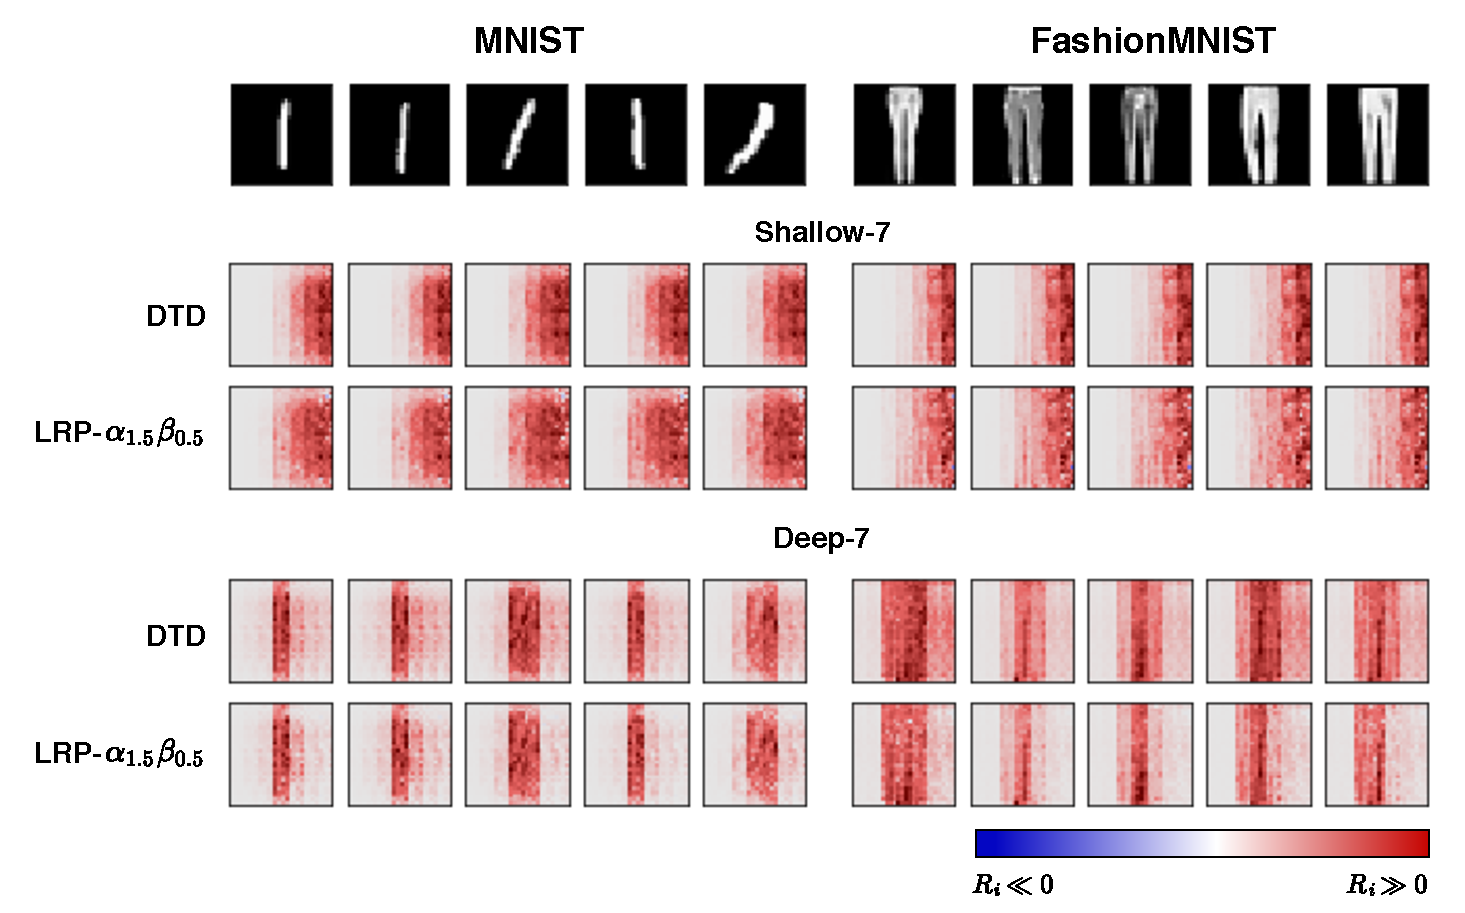
\includegraphics[width=0.8\textwidth]{sketch/class_1_comparison}
\caption{Relevance heatmaps of MNIST \textit{Class 1} and FashionMNIST \textit{Class Trouser} samples from \rnncellseq{Shallow}{7} and \rnncellseq{Deep}{7} explained by DTD and $\lrpp$. \heatmapscaleexplain }
\label{fig:class_1_comparison}
\end{figure}

\addfigure{\ref{fig:class_1_comparison}} presents relevance heatmaps of MNIST \textit{Class 1} and FashionMNIST \textit{Class Trouser} samples. These samples were chosen to emphasize the impact of RNN architecture on DTD and LRP explanation. In particular,  as can be seen from the figure, these samples have $\x_{t'}$ containing actual content  primarily locating at the center, or middle of the sequence. Hence, relevance heatmaps should be highlighted at $\x_{t'}$ and possibly its neighbors.  As expected, we can see \rnncellseq{Deep}{7} produces sound explanations in which the heatmaps have high intensity value where $\x_{t'}$ approximately locate, while \rnncellseq{Shallow}{7} mainly assigns relevance quantities to $\x_{t}$ for $t \approx T$. 

\addfigure{\ref{fig:exp1_dist_plot}} further shows a quantitive evidence of this wrong propagation issue of DTD and $\lrpp$. Here, distributions of relevance scores derived by the methods from \rnncellseq{Shallow}{7} and \rnncellseq{Deep}{7} are plotted across time step $t = \{ 1, \dots, 7 \}$. The distributions are computed from all test samples in MNIST \textit{Class 1} and FashionMNIST \textit{Class Trouser} respectively. The plots also include distribution of pixel intensity values.  We can see that the relevance distributions from \rnncellseq{Deep}{7} align with the data distributions, while  the distributions from \rnncellseq{Shallow}{7} ones diverge with significant margin. Approximately,  one can see that \rnncellseq{Shallow}{7} distributes more than 90\% of relevance scores to the last 3 steps, namely $\x_5$, $\x_6$ and $\x_7$.


 \begin{figure}[!htb]
\centering
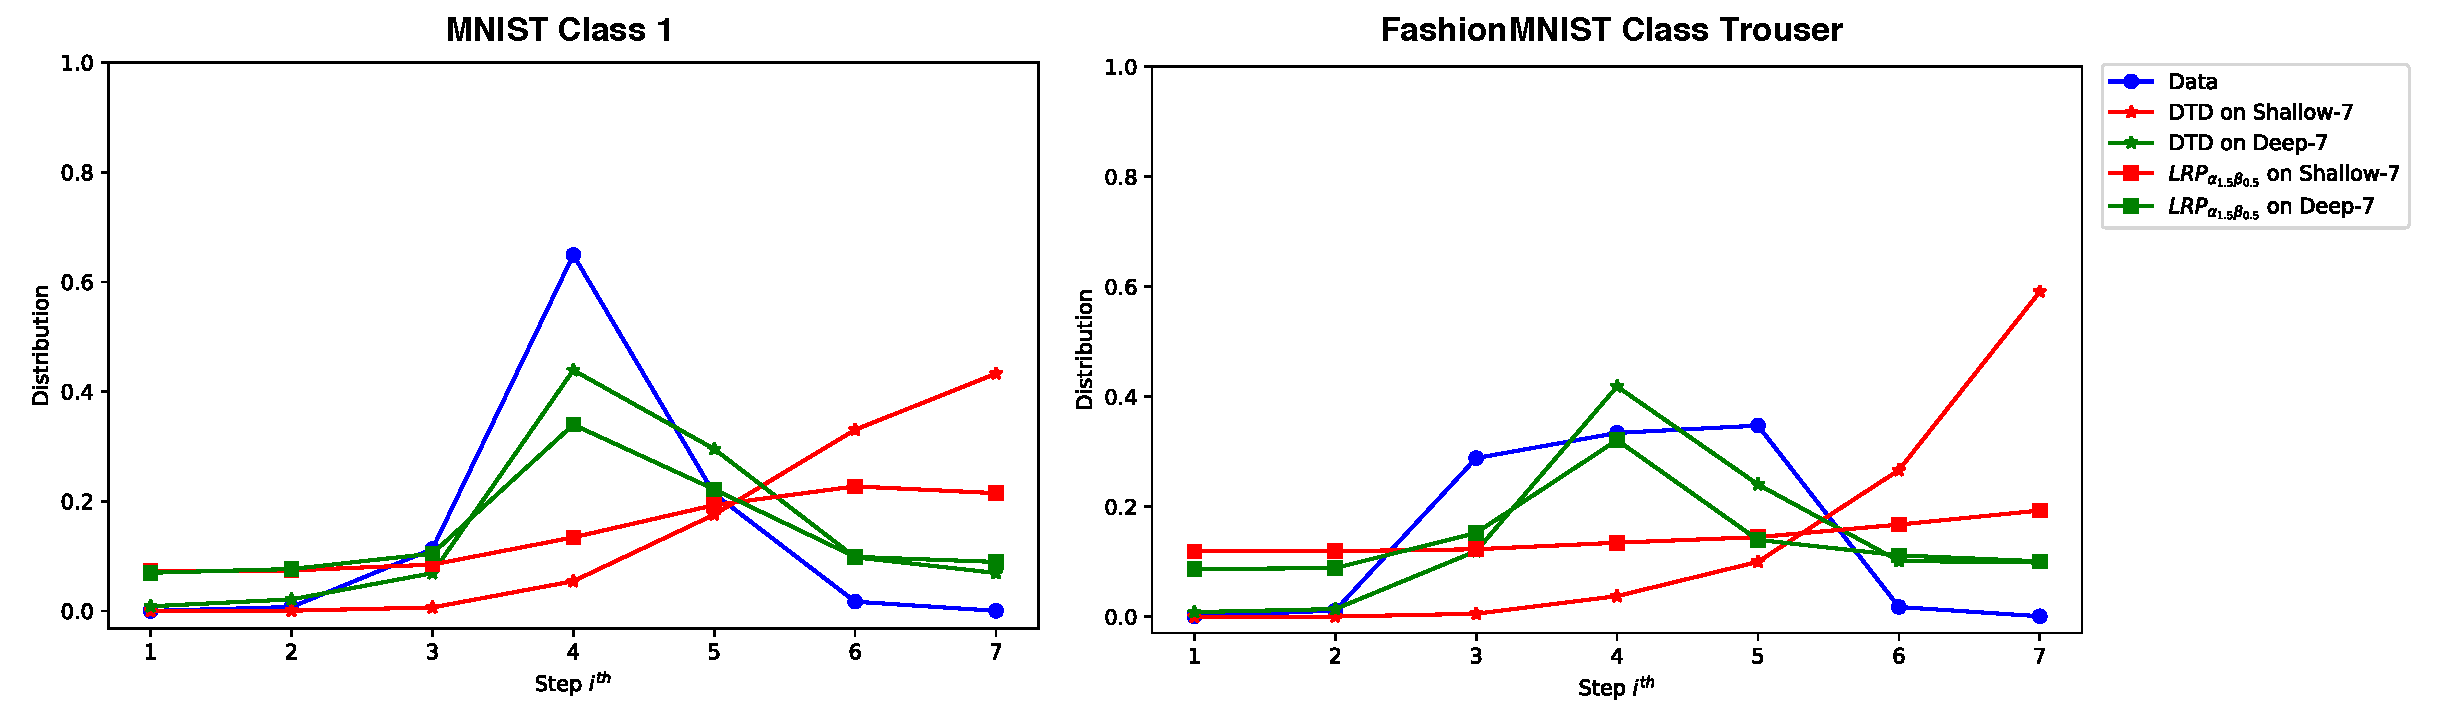
\includegraphics[width=\textwidth]{sketch/exp1_dist_plot}
\caption{Distribution of pixel intensity, relevance quantities from \rnncellseq{Shallow}{7} and \rnncellseq{Deep}{7} propagated by DTD and $\lrpp$ and averaged over MNIST \textit{Class 1} and FashionMNIST\textit{Class Trouser} test population.} 
\label{fig:exp1_dist_plot}
\end{figure}

\subsection{Summary}\todo{review}
Results from this first experiment seem to suggest that choice of RNN architectures has an impact on quality of its explanation.  In particular,  as presented in \addfigure{\ref{fig:class_1_comparison}} and \addfigure{\ref{fig:exp1_dist_plot}}, quality of deep Taylor decomposition(DTD) explanation is significantly influenced by the architecture. In contrast, we do see such notable effect from sensitivity analysis(SA) and guided backprop(GB) method.  In the following experiment, I am going to present a methodical evaluation of this impact in detail.


\section{Experiment 2 : Majority Sample Sequence Classification} \label{sec:exp2}
   
 \begin{figure}[!htb]
\centering
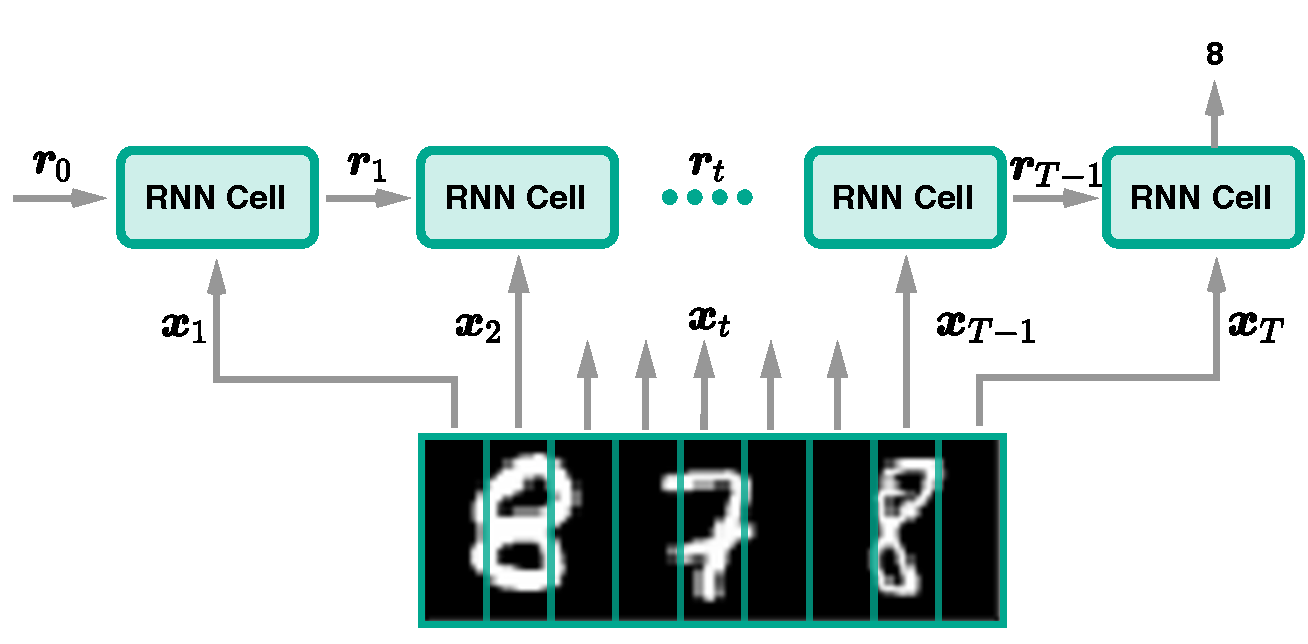
\includegraphics[width=0.8\textwidth]{sketch/artificial_problem_3digits}
\caption{Majority Sample Sequence Classification(MAJ) problem.} 
\label{fig:artificial_problem_3digits}
\end{figure}

\subsection{Problem Formulation} \label{sec:exp2_prob_formulate}
When neural networks are trained, one can apply explantation techniques to the models to get relevance heatmaps of samples.  The heatmap of sample $\x$ illustrates important features in $x$ that the trained network utilizes to perform its objective prediction,  such as classification.  Therefore, one needs to know the ground truth of these latent features in order to methodologically evaluate how well the model distributes  relevance scores to the input space, in other words, how the model can be explained. However,  this knowledge is not trivial to find as it is an incident from the optimization process in high-dimensional space that we in fact seek to understand.

To alleviate this challenge, we instead  constructed another artificial classification problem where RNNs are trained to classify  the majority group in a sequence $\x$, $(\x_t )_{t=1}^{T}$. Consider MNIST. $\x$ is constructed as follows: each original sample $\widetilde{\x} \in \mathbb{R}^{28,28}$, we randomly selected 2 additional samples : one from the same class of $\widetilde{\x}$ and the other one from a different class. Then, these 3 samples are concatenated in random order yielding a sample $\x \in \mathbb{R}^{28,84}$.  \addfigure{\ref{fig:artificial_problem_3digits}} illustrates the construction and the objective classification. Given $\x = \{ 8, 7, 8\}$, the classification result is ``8"".  We call this problem as MNIST-MAJ when $\x$ are constructed from MNIST samples and the same for FashionMNIST-MAJ.

By construction, we already know blocks of digit/item that belong to the majority group. More precisely, we know time step $t'$ that are parts of those blocks, hence, we can use this information to  quantitively evaluate  how well RNN architectures can propagate relevance quantities to the input, in other words, how well they can be explained.


As discussed in the previous experiment that some DTD and $\lrpp$ heatmaps from the Deep architecture were not as good as the others. This seems to suggest that the architecture might not have enough capability to extract proper representations from FashionMNIST samples, causing the incorrect propagation issue on such heatmaps. 

Hence, apart of Shallow and Deep architecture, we also introduced another two architectures, namely DeepV2 and ConvDeep. The DeepV2 cell has one more layer after the first fully-connected layer than the Deep cell. On the other hand, the ConvDeep cell instead employs a sequence of convolutional and pooling operation and a fully-connected layer between the input layer and the internal layer. \addfigure{\ref{fig:deep_conv_arch}} shows details of the new architectures. 


%\subsection{Setting}
%Two variations of \rnncell{Deep} cell are also experimented, namely \rnncell{DeepV2} and \rnncell{ConvDeep}, shown on \addfigure{\ref{fig:deep_conv_arch}}. The former has one additional layer \circled{1"} with dropout regularization  between \circled{1'}. On the other hand, the latter replaces fully connected layers between \circled{1} and \circled{3} with 2 convolutional and max pooling layers, \Big[\circled{C1}, \circled{P1}\Big] and \Big[\circled{C2},\circled{P2}\Big].

\begin{figure}[!htb]
\centering

\subfloat[DeepV2\label{fig:deep_4l_network}]{%
       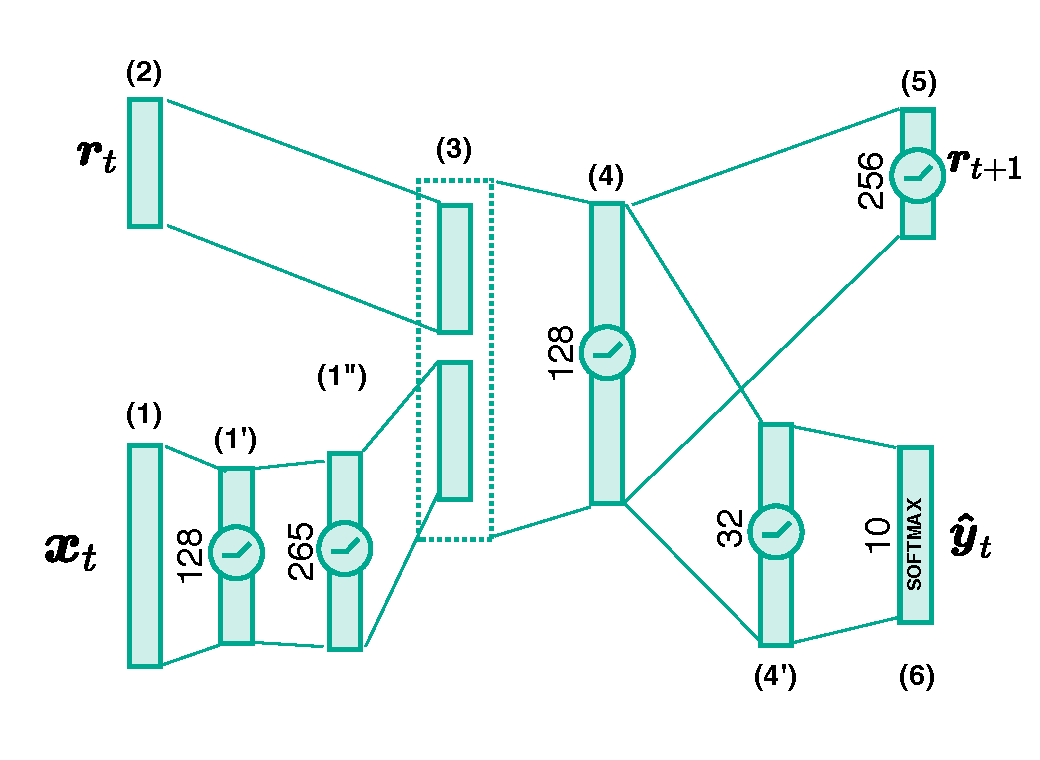
\includegraphics[width=0.48\textwidth]{sketch/deep_v2_arch}
     }
     \hfill
     \subfloat[ConvDeep\label{fig:convdeep_4l_network}]{%
       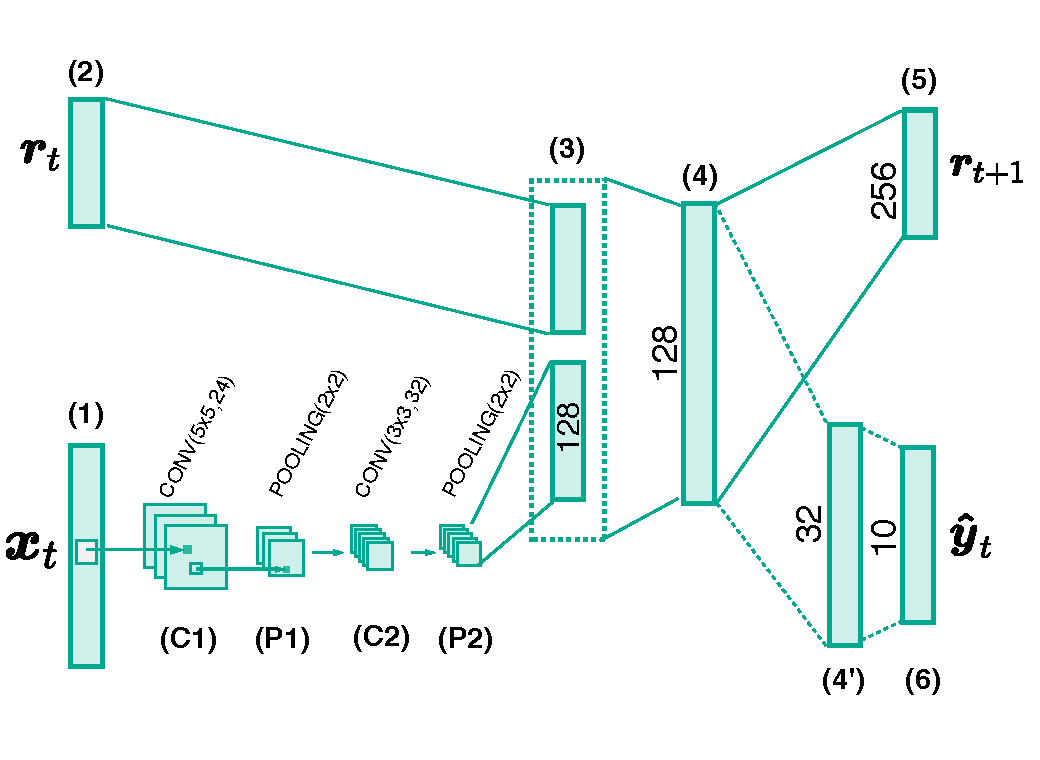
\includegraphics[width=0.48\textwidth]{sketch/convdeep_arch}
     }

\caption{DeepV2 and ConvDeep cell architecture with number of neurons at each layer depicted.}
\label{fig:deep_conv_arch}
\end{figure}

Lastly, despite the fact that  our implementation is readily to apply on different sequence lengths,  we conducted the experiment with only sequence length $T=12$, or $(\x_t \in \mathbb{R}^{28,7})_{t=1}^{12}$. This is mainly due to computational resources and time constraint we had. Consequently, slightly abusing the name convention proposed in Section \ref{sec:exp1}, we are going to write only the name of architecture without explicitly stating the sequence length towards the end of this chapter.


\subsection{Evaluation Methodology}
\label{sec:evaluation_med}
From the problem construction, we know that relevance quantities should  be primarily assigned to blocks that belong to the majority group. This construction enables us to both directly examine quality of produced relevance heatmaps visually as well as quantitative evaluation.  In particular, for qualitative inspections, we constructed training and testing data based on the original training and testing split that \cite{LeCunMNISThandwrittendigit2010} and \cite{XiaoFashionMNISTNovelImage2017} proposed and trained with setting described in Section \ref{sec:setup}.

\subsubsection{Quantitative Evaluation}
A straightforward way to quantitatively evaluate results is to calculate proportion of relevance distributed to pixels that are contained in the blocks of the majority group digit/item. However, this measurement has a shortcoming where architectures can achieve high score if they distribute relevance to only one of the correct blocks. Hence, we then propose to use \textit{cosine similarity} instead. The cosine similarity is computed from  a  binary  vector $\patvector{m} \in \mathbb{R}^3$  whose values represent correctness of the blocks and a vector $\patvector{\upsilon} \in \mathbb{R}^3$ of relevance percentage distributed to the blocks. 

\begin{align}
\cos (\patvector{m}, \patvector{\upsilon}) = \frac{ \patvector{m} \cdot \patvector{\upsilon}}{ || \patvector{m}  ||_2 ||\patvector{\upsilon}   ||_2}	
\end{align}

As illustrated in \addfigure{\ref{fig:quantitative_evaluation}}, the percentage of correctly distributed relevance can be significantly high although the relevance heatmap does not show any highlight at the left most block of ``0". Therefore, using cosine similarity is more reasonable. In fact, the propagation needs to be equally balanced between the two blocks in order to achieve the highest score, ``1". For $\lrpp$ heatmaps, we ignore negative relevance and set it to zero before computing cosine similarity.

\begin{figure}[!htb]
\centering
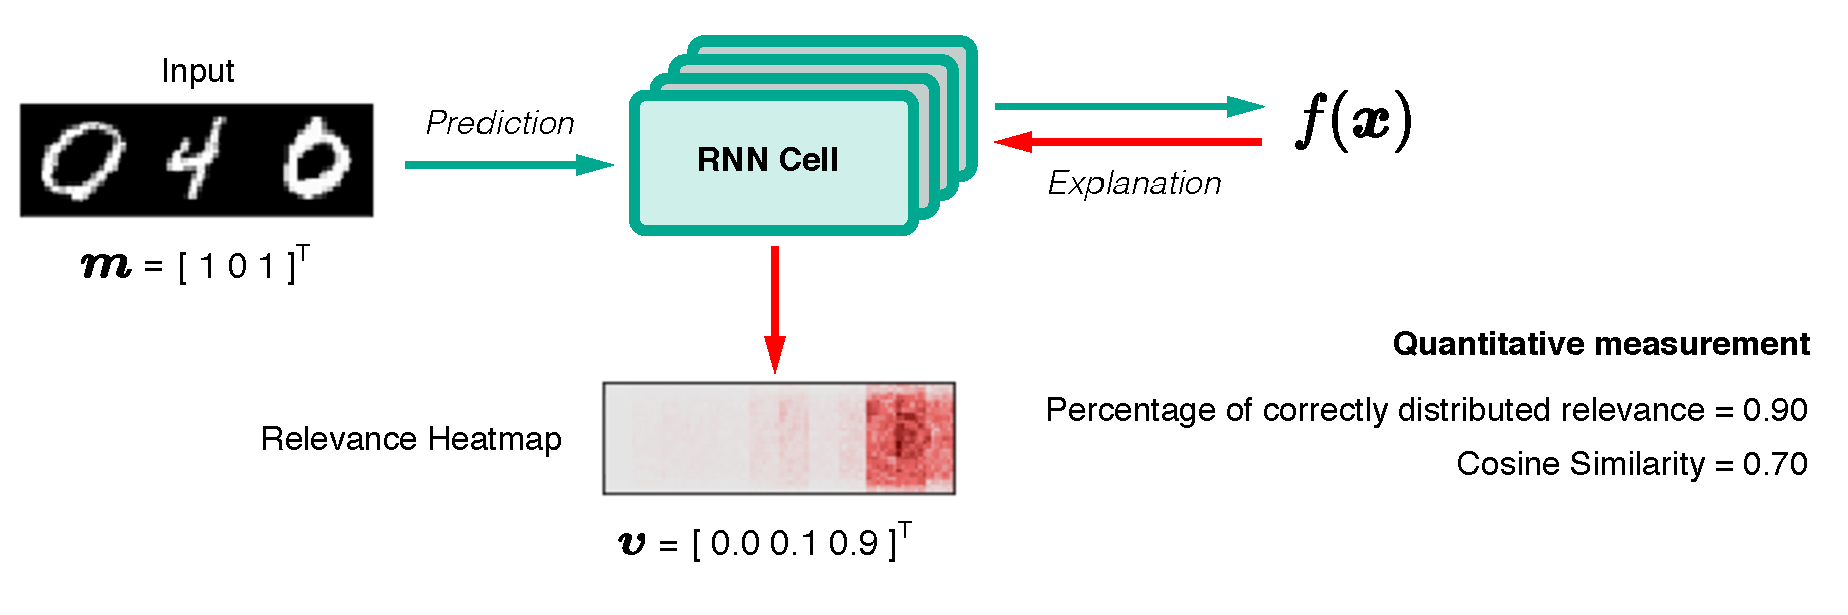
\includegraphics[width=\textwidth]{sketch/quantitative_evaluation}
\caption{Comparison of 2 quantitative measurements} 
\label{fig:quantitative_evaluation}
\end{figure}

\subsubsection{Statistical Evaluation}
To reduce variations possibly introduced by, for example variable initialization, we conducted quantitatively evaluations through $k$-fold cross-validation where we combined  training and testing set together before spliting into $k$ folds. Each fold is used as the testing set once. For each cross-validation iteration, we average the cosine similarity across testing samples. The final result is then averaged from folds' statistics.  To keep the same proportion of training and testing data, we chose $k=7$. 

\todo{ check whether we need it: 
It is also possible that some architectures might perform similarly and the difference is not visually observed. For such scenarios, we will use one-way ANOVA on statistics of cosine similarity and pairwise Tukey Honest Significant Difference (HSD) as a post-hoc test to verify whether there are statistically significant results. We use significance level at $0.05$. Dataset is considered as a confounding variable. This procedure is conducted separately for each explanation method.
}



 %Table x show accuracy sf

\subsection{Result}

\renewcommand{\arraystretch}{1.5}
\begin{table}[h]
\begin{center}
\begin{tabular}{lc|c|c|}
\cline{3-4}
& &
\multicolumn{2}{c|}{\parbox{3.5cm}{ \vskip 1mm \centering \textbf{Accuracy} \vskip 1mm}} \\ \hline
\multicolumn{1}{|l|}{\textbf{Cell architecture}} & \textbf{No. variables} & \textbf{MNIST-MAJ} & \textbf{FashionMNIST-MAJ} \\ \hline
\multicolumn{1}{|l|}{Shallow}    & 184,330          & 98.12\% & 90.00\% \\ 
\multicolumn{1}{|l|}{Deep}       & 153,578           & 98.16\% & 89.81\% \\ 
 \multicolumn{1}{|l|}{DeepV2}     & 161,386        & 98.26\% & 90.57\% \\
\multicolumn{1}{|l|}{ConvDeep}   & 151,802       & 99.22\% & 92.87\%  \\ \hline 
\end{tabular}

\end{center}
\caption{Number of trainable variables and model accuracy from architectures trained on MNIST-MAJ and FashionMNIST-MAJ with sequence length $T=12$.}
\label{tab:maj_rnn_model_acc}
\end{table}
\renewcommand{\arraystretch}{1}

 \begin{figure}[!htb]
\centering
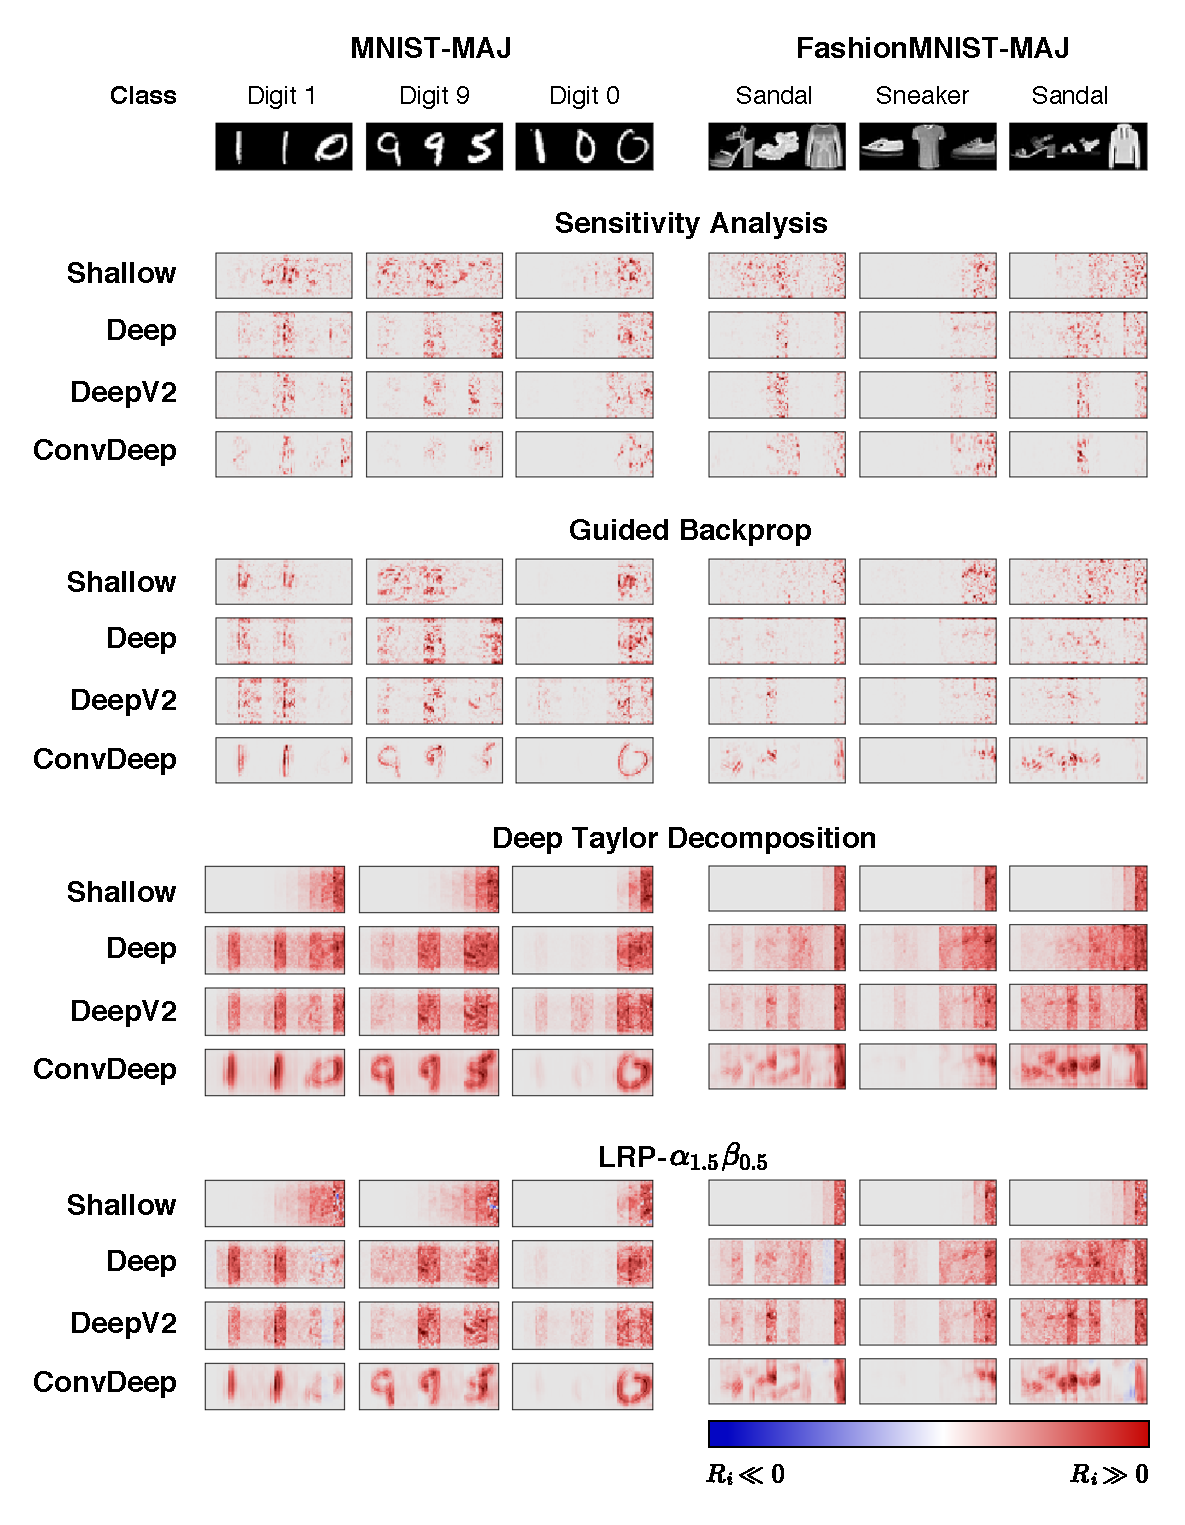
\includegraphics[width=\textwidth]{sketch/heatmap_msc_for_thesis}
\caption{Relevance heatmaps produced by different explanation techniques on Shallow, Deep, DeepV2 and ConvDeep architecture trained on MNIST-MAJ and FashionMNIST-MAJ with sequence length $T=12$. \heatmapscaleexplain } 
\label{fig:heatmap_msc_mix_for_thesis}
\end{figure}

Table \ref{tab:maj_rnn_model_acc} shows number of trainable variables and accuracy of the trained models. These trained models have equivalent number of variables and accuracy, hence comparing heatmaps of these models is a fair evaluation.

\addfigure{\ref{fig:heatmap_msc_mix_for_thesis}} shows that the deeper architecture improves relevance propagation, or easier to be explained. In particular, we can see that fewer relevant scores distributed to irrelevant region are gradually reduced from Shallow to ConvDeep architecture. This effect happens across all explanation methods. This result further supports the evidence discussed in Section \ref{sec:exp1}.  Moreover, although relevance heatmaps from \rnncell{Shallow}, \rnncell{Deep}, and \rnncell{DeepV2} generally look noisy, increasing the depth of architecture seems to reduce the noise in the heatmaps as well.   On the other hand, \rnncell{ConvDeep} does not  only properly assign relevance quantities to the right time steps, but its heatmaps contains $\x$'s features that we can not easily observe from the other architectures. For example, GB and $\lrpp$ heatmaps of Digit 1 and Sandal samples are cases.

\clearpage

 \begin{figure}[!hbt]
\centering
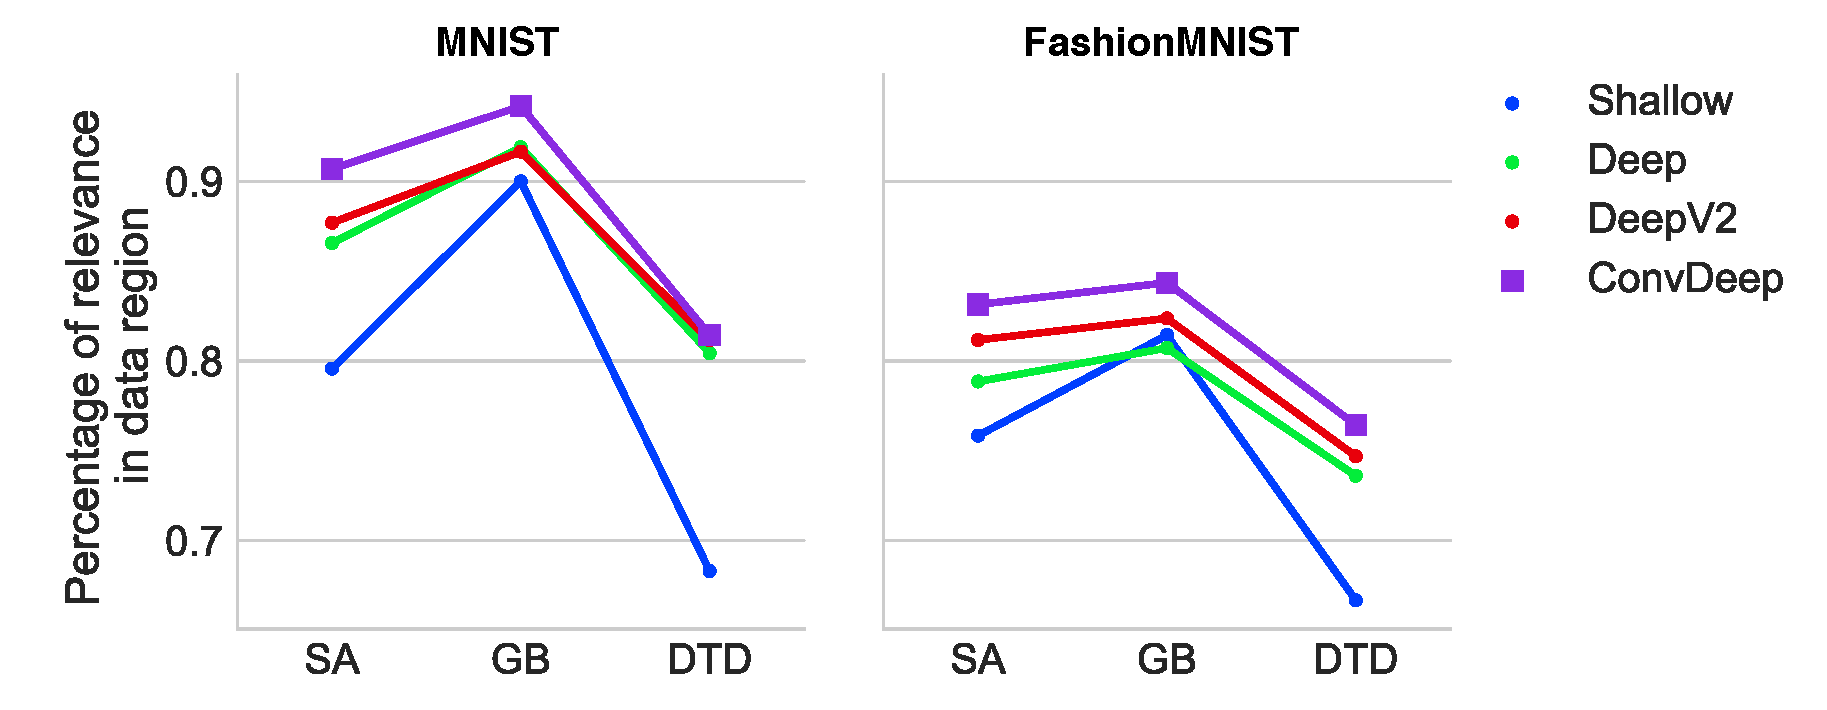
\includegraphics[width=\textwidth]{sketch/rel_dist_maj_3_samples_thesis}
\caption{Average cosine similarity from different explanation techniques and Shallow, Deep, DeepV2 and ConvDeep architecture. The values are averaged from cross-validation results and the vertical lines depicted 95\% confidence interval. The baseline is the Shallow architecture depicted by the blue line.\todo{link accuracy to appendix}} 
\label{fig:rel_dist_maj_3_samples_thesis}
\end{figure}

\addfigure{\ref{fig:rel_dist_maj_3_samples_thesis}} presents a quantitive  evaluation of the impact from the depth of architecture to the explanation. The measurement is cosine similarity between a mark vector $\boldsymbol{m} \in \mathbb{R}^3$ and an aggregated relevance to blocks of digit/item vector $\boldsymbol{\upsilon \in \mathbb{R}^3 }$ and averaged through $7$-fold cross-validation procedure as described in Section \ref{sec:evaluation_med}. Results from the figure indicate that the depth of architecture indeed improves quality of the explanations. In particular, the percentage of correct relevance assignment of each explanation technique increases as more layers introduced. This effect can be seen clearly from the result of FashionMNIST-MAJ. Additionally, we can observe that the difference of cosine similarity between the baseline, \rnncell{Shallow}, and the other  architectures changes with different proposition across methods. In particular, we see the difference from DTD and $\lrpp$ are much larger than the other methods. This implies that some explanation methods are more sensitive to architecture configuration than the others.


\todo{hypo : pair wise statistical testing}

\subsection{Summary}
The outcome of this experiment quantitively confirms that the depth of architecture has impacts on explanation of the model. It also shows that  the depth of architecture affects explanation in different level on different methods. More precisely, quality of explanations produced by deep Taylor decomposition(DTD) and Layer-Wise Relevance Propagations(LRP) technique are more sensitive to the architecture of the explained model than sensitivity analysis(SA) and guided backprop(GB) method.

Nonetheless, we have also observed that significant amount of relevance scores are distributed to irrelevant regions, for example, consider Digit ``9" sample on \addfigure{\ref{fig:heatmap_msc_mix_for_thesis}}. Therefore, we are going to purpose several improvements to the problem.

